\documentclass[tikz,border=5pt]{standalone}
\usepackage{pgfplots}
\usepgfplotslibrary{groupplots}
\pgfplotsset{compat=1.18}

\definecolor{corba}{HTML}{365FB3}
\definecolor{punt}{HTML}{B91C1C}
\definecolor{tangent}{HTML}{6B7280}

\begin{document}
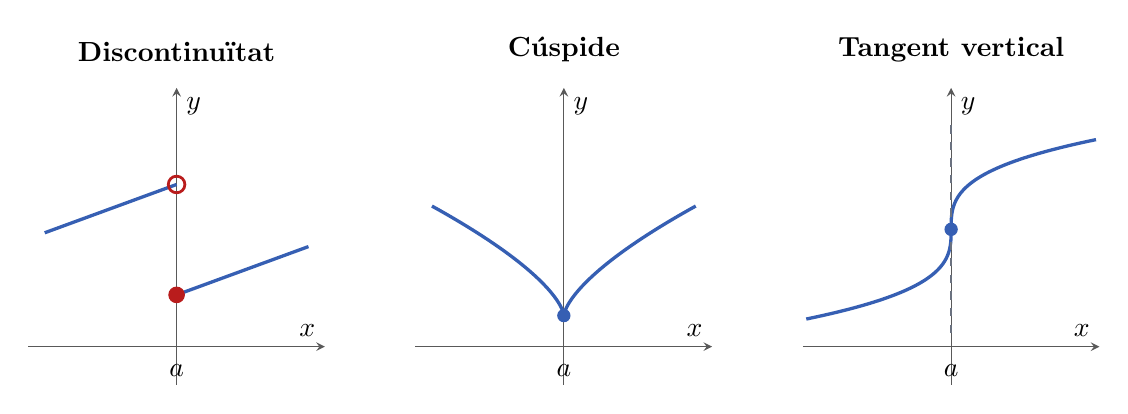
\begin{tikzpicture}
  \begin{groupplot}[
    group style={group size=3 by 1, horizontal sep=1.15cm},
    width=5.35cm,
    height=5.35cm,
    axis lines=middle,
    xmin=-2.25,
    xmax=2.25,
    ymin=-0.55,
    ymax=3.75,
    xlabel={$x$},
    ylabel={$y$},
    xtick=\empty,
    ytick=\empty,
    axis line style={black!65},
    tick style={black!65},
    clip=false,
  ]
    % Discontinuïtat de salt.
    \nextgroupplot[title={\textbf{Discontinuïtat}}]
      \addplot[corba, very thick, domain=-2:0, samples=80]
        {0.35*x+2.35};
      \addplot[corba, very thick, domain=0:2, samples=80]
        {0.35*x+0.75};
      \addplot[
        only marks,
        mark=o,
        mark size=3pt,
        mark options={draw=punt, fill=white, line width=1pt}
      ] coordinates {(0,2.35)};
      \addplot[
        only marks,
        mark=*,
        mark size=2.8pt,
        mark options={draw=punt, fill=punt}
      ] coordinates {(0,0.75)};
      \node[anchor=north] at (axis cs:0,-0.12) {$a$};

    % Cúspide: pendents laterals infinites de signe contrari.
    \nextgroupplot[title={\textbf{Cúspide}}]
      \addplot[corba, very thick, domain=-2:0, samples=140]
        {(-x)^(2/3)+0.45};
      \addplot[corba, very thick, domain=0:2, samples=140]
        {x^(2/3)+0.45};
      \addplot[only marks, mark=*, mark size=2.2pt, corba]
        coordinates {(0,0.45)};
      \node[anchor=north] at (axis cs:0,-0.12) {$a$};

    % Tangent vertical: corba paramètrica (t^3,t+1.7).
    \nextgroupplot[title={\textbf{Tangent vertical}}]
      \addplot[corba, very thick, domain=-1.3:1.3, samples=150]
        ({x^3},{x+1.7});
      \addplot[tangent, dashed, thick] coordinates {(0,0.2) (0,3.25)};
      \addplot[only marks, mark=*, mark size=2.2pt, corba]
        coordinates {(0,1.7)};
      \node[anchor=north] at (axis cs:0,-0.12) {$a$};
  \end{groupplot}
\end{tikzpicture}
\end{document}
